\documentclass[
a4paper,
10pt,fleqn,
oneside,openright
]{memoir} 	% Openright aabner kapitler paa hoejresider (openany begge)

%%psw%%
\usepackage{titletoc}
%\titlecontents{}% <section-type>
%  [0pt]% <left>
%  {\bfseries}% <above-code>
%  {\chaptername\ \thecontentslabel:\quad}% <numbered-entry-format>
%  {}% <numberless-entry-format>
%  {\hfill\contentspage}% <filler-page-format>
\setlrmarginsandblock{3cm}{3cm}{*}
\setulmarginsandblock{3cm}{4cm}{*}
% space for header material and footer material
\setheadfoot{14mm}{7mm}
% spacings within the header
\setheaderspaces{*}{3mm}{*}

\checkandfixthelayout[nearest] 						% Oversaetter vaerdier til brug for andre pakker

% \setlrmarginsandblock{3.5cm}{2.5cm}{*}		% \setlrmarginsandblock{Indbinding}{Kant}{Ratio}
% \setulmarginsandblock{2.5cm}{3.0cm}{*}		% \setulmarginsandblock{Top}{Bund}{Ratio}

%	¤¤ Afsnitsformatering ¤¤ %
\setlength{\parindent}{0mm}           		% Stoerrelse af indryk
\setlength{\parskip}{3mm}          			% Afstand mellem afsnit ved brug af double Enter
\linespread{1,1}							% Linie afstand

\usepackage{longtable}

%%%% PACKAGES %%%%
\usepackage{listings}
\usepackage{nameref}
% ¤¤ Oversaettelse og tegnsaetning ¤¤ %
\usepackage[utf8]{inputenc}					% Input-indkodning af tegnsaet (UTF8)
\usepackage[danish]{babel}					% Dokumentets sprog
\usepackage[T1]{fontenc}					% Output-indkodning af tegnsaet (T1)
\usepackage{ragged2e,anyfontsize}			% Justering af elementer
\usepackage{fixltx2e}						% Retter forskellige fejl i LaTeX-kernen
\usepackage{tabularx}
\usepackage{booktabs}
\usepackage{siunitx}
\usepackage{wrapfig}
																			
% ¤¤ Figurer og tabeller (floats) ¤¤ %
%\usepackage{tikz} % Graphical tool

\usepackage{graphicx} 						% Haandtering af eksterne billeder (JPG, PNG, PDF)
\usepackage{multirow}                		% Fletning af raekker og kolonner (\multicolumn og \multirow)
\usepackage{colortbl} 						% Farver i tabeller (fx \columncolor, \rowcolor og \cellcolor)
\usepackage[xcdraw]{xcolor}
%\usepackage[dvipsnames]{xcolor}				% Definer farver med \definecolor. Se mere: %http://en.wikibooks.org/wiki/LaTeX/Colors
\usepackage{flafter}						% Soerger for at floats ikke optraeder i teksten foer deres reference
\let\newfloat\relax 						% Justering mellem float-pakken og memoir
\usepackage{float}							% Muliggoer eksakt placering af floats, f.eks. \begin{figure}[H]
\usepackage{adjustbox}				% Muliggoer left og right placering af billeder
%\usepackage{eso-pic}						% Tilfoej billedekommandoer paa hver side
\usepackage{wrapfig}						% Indsaettelse af urer omsvoebt af tekst. \begin{wrapfigure}{Placering}{Stoerrelse}
%\usepackage{multicol}         	        	% Muliggoer tekst i spalter
%\usepackage{rotating}						% Rotation af tekst med \begin{sideways}...\end{sideways}
%\usepackage{caption} 						% Giver mulighed for at redigere bredden på captions, hvis dit billede er mindre end caption

% ¤¤ Matematik mm. ¤¤
\usepackage{amsmath,amssymb,stmaryrd} 		% Avancerede matematik-udvidelser
\usepackage{mathtools}						% Andre matematik- og tegnudvidelser
\usepackage{textcomp}                 		% Symbol-udvidelser (f.eks. promille-tegn med \textperthousand )
\usepackage{siunitx}						% Flot og konsistent praesentation af tal og enheder med \si{enhed} og \SI{tal}{enhed}
\sisetup{output-decimal-marker = {,}}		% Opsaetning af \SI (DE for komma som decimalseparator) 
%\usepackage[version=3]{mhchem}
\usepackage{fix-cm} % Fix for cm 				% Kemi-pakke til flot og let notation af formler, f.eks. \ce{Fe2O3}
%\usepackage{rsphrase}						% Kemi-pakke til RS-saetninger, f.eks. \rsphrase{R1}

% ¤¤ Referencer og kilder ¤¤ %
\usepackage[danish]{varioref}				% Muliggoer bl.a. krydshenvisninger med sidetal (\vref)
\usepackage[square, numbers, authoryear, super]{natbib}
%\usepackage[backend=bibtex]{biblatex}
\bibliographystyle{Projektrapport/natbib}
%\usepackage[square,numbers]{natbib}							% Udvidelse med naturvidenskabelige citationsmodeller
%\usepackage{xr}							% Referencer til eksternt dokument med \externaldocument{<NAVN>}
%\usepackage{glossaries}					% Terminologi- eller symbolliste (se mere i Daleifs Latex-bog)

% ¤¤ Misc. ¤¤ %
\usepackage{listings}						% Placer kildekode i dokumentet med \begin{lstlisting}...\end{lstlisting}

\usepackage{lipsum}							% Dummy text \lipsum[..]
\usepackage[shortlabels]{enumitem}			% Muliggoer enkelt konfiguration af lister
\usepackage{pdfpages}						% Goer det muligt at inkludere pdf-dokumenter med kommandoen \includepdf[pages={x-y}]{fil.pdf}	

\pdfoptionpdfminorversion=6					% Muliggoer inkludering af pdf dokumenter, af version 1.6 og hoejere
\pretolerance=2500 							% Justering af afstand mellem ord (hoejt tal, mindre orddeling og mere luft mellem ord)

% Kommentarer og rettelser med \fxnote. Med 'final' i stedet for 'draft' udloeser hver note en error i den faerdige rapport.
\usepackage[footnote,draft,danish,silent,nomargin]{fixme}		


%%%% CUSTOM SETTINGS %%%%

% ¤¤ Marginer ¤¤ %

% marginer roder man ikke med manuelt nede i dokumentet /daleif


% ¤¤ TOC ¤¤ %

\setpnumwidth{3em}
\setrmarg{3.55em}



% ¤¤ Litteraturlisten ¤¤ %

% \bibpunct[,]{[}{]}{;}{a}{,}{,} 				% Definerer de 6 parametre ved Harvard henvisning (bl.a. parantestype og seperatortegn)
%\bibliographystyle{bibtex/harvard}			% Udseende af litteraturlisten.

% ¤¤ Indholdsfortegnelse ¤¤ %
\setsecnumdepth{paragraph}		 			% Dybden af nummerede overkrifter (part/chapter/section/subsection)
\maxsecnumdepth{paragraph}					% Dokumentklassens graense for nummereringsdybde
\settocdepth{paragraph} 					% Dybden af indholdsfortegnelsen

% ¤¤ Lister ¤¤ %
\setlist{
  topsep=0pt,								% Vertikal afstand mellem tekst og listen
  itemsep=-1ex,								% Vertikal afstand mellem items
} 

% ¤¤ Visuelle referencer ¤¤ %
\usepackage[colorlinks]{hyperref}			% Danner klikbare referencer (hyperlinks) i dokumentet.
\hypersetup{colorlinks = true,				% Opsaetning af farvede hyperlinks (interne links, citeringer og URL)
    linkcolor = black,
    citecolor = black,
    urlcolor = black
}

% ¤¤ Opsaetning af figur- og tabeltekst ¤¤ %
\captionnamefont{\small\bfseries\itshape}	% Opsaetning af tekstdelen ('Figur' eller 'Tabel')
\captiontitlefont{\small}					% Opsaetning af nummerering
\captiondelim{. }							% Seperator mellem nummerering og figurtekst
\hangcaption								% Venstrejusterer flere-liniers figurtekst under hinanden
\captionwidth{\linewidth}					% Bredden af figurteksten
\setlength{\belowcaptionskip}{0pt}			% Afstand under figurteksten
		
% ¤¤ Opsaetning af listings ¤¤ %
\definecolor{commentGreen}{RGB}{34,139,24}
\definecolor{stringPurple}{RGB}{155,104,2}
\definecolor{ase_blue}{RGB}{10,55,136}
\definecolor{bluekeywords}{rgb}{0,0,1}
\definecolor{types}{rgb}{0.17,0.57,0.68}
\definecolor{redstrings}{rgb}{0.64,0.08,0.08}

\lstset{language=csh,					% Sprog
	captionpos=b,
	showspaces=false,
	showtabs=false,
	breaklines=true,
	showstringspaces=false,
	breakatwhitespace=true,
	escapeinside={(*@}{@*)},
	commentstyle=\color{commentGreen},		% Opsaetning af kommentarer
	morecomment=[l]{//}, 					%use comment-line-style!
	morecomment=[s]{/*}{*/}, 				%for multiline comments
	stringstyle=\color{stringPurple},		% Opsaetning af strenge
	keywordstyle=\color{bluekeywords},
	stringstyle=\color{redstrings},
	basicstyle=\ttfamily\small,
	showstringspaces=false,					% Mellemrum i strenge enten vist eller blanke
	numbers=left, numberstyle=\tiny,		% Linjenumre
	extendedchars=true, 					% Tillader specielle karakterer
	columns=flexible,						% Kolonnejustering
	breaklines, breakatwhitespace=true,		% Bryd lange linjer
	morekeywords={  abstract, event, new, struct,
                as, explicit, null, switch,
                base, extern, object, this,
                bool, false, operator, throw,
                break, finally, out, true,
                byte, fixed, override, try,
                case, float, params, typeof,
                catch, for, private, uint,
                char, foreach, protected, ulong,
                checked, goto, public, unchecked,
                class, if, readonly, unsafe,
                const, implicit, ref, ushort,
                continue, in, return, using,
                decimal, int, sbyte, virtual,
                default, interface, sealed, volatile,
                delegate, internal, short, void,
                do, is, sizeof, while,
                double, lock, stackalloc,
                else, long, static,
                enum, namespace, string},
}


% ¤¤ Navngivning ¤¤ %
\addto\captionsdanish{
	\renewcommand\appendixname{Appendiks}
	\renewcommand\contentsname{Indholdsfortegnelse}	
	\renewcommand\appendixpagename{Appendiks}
	\renewcommand\appendixtocname{Appendiks}
	\renewcommand\cftchaptername{\chaptername~}				% Skriver "Kapitel" foran kapitlerne i indholdsfortegnelsen
	\renewcommand\cftappendixname{\appendixname~}			% Skriver "Appendiks" foran appendiks i indholdsfortegnelsen
}

% ¤¤ Kapiteludssende ¤¤ %
\definecolor{numbercolor}{gray}{0.7}		% Definerer en farve til brug til kapiteludseende
\newif\ifchapternonum

\makechapterstyle{jenor}{					% Definerer kapiteludseende frem til ...
  \renewcommand\chapterheadstart{}
  \renewcommand\beforechapskip{0pt}
  \renewcommand\printchaptername{}
  \renewcommand\printchapternum{}
  \renewcommand\printchapternonum{\chapternonumtrue}
  \renewcommand\chaptitlefont{\fontfamily{pbk}\fontseries{db}\fontshape{n}\fontsize{20}{30}\selectfont\raggedright}
  \renewcommand\chapnumfont{\fontfamily{pbk}\fontseries{m}\fontshape{n}\fontsize{0.6in}{0in}\selectfont\color{numbercolor}}
  \renewcommand\printchaptertitle[1]{%
    \noindent
    \ifchapternonum
    \begin{tabularx}{\textwidth}{X}
    {\let\\\newline\chaptitlefont ##1\par} 
    \end{tabularx}
    \par\vskip-2.5mm\hrule
    \else
    \begin{tabularx}{\textwidth}{Xl}
    {\parbox[b]{\linewidth}{\chaptitlefont ##1}} & \raisebox{-15pt}{\chapnumfont \thechapter}
    \end{tabularx}
    \par\vskip2mm\hrule
    \fi
  }
}											% ... her

\chapterstyle{jenor}						% Valg af kapiteludseende - Google 'memoir chapter styles' for alternativer
%\chapterstyle{southall}{%
%	 \renewcommand{\afterchaptertitle}{{%
%	 		\par\offinterlineskip\hbox{\hspace*{-\marginparwidth}\rule{0.7\textwidth}{5pt}}}}
%}
%\renewcommand*{\chapterheadendvskip}{\vspace{10cm}}

%\chapterstyle{tandh}

% Afstand omkring titler
\usepackage[compact]{titlesec}
\titlespacing*{\section}{0pt}{5pt}{0pt}
\titlespacing*{\subsection}{0pt}{5pt}{0pt}
\titlespacing*{\subsubsection}{0pt}{5pt}{0pt}

% ¤¤ Sidehoved ¤¤ %

\makepagestyle{Uni}							% Definerer sidehoved og sidefod udseende frem til ...
\makepsmarks{Uni}{%
	\createmark{chapter}{left}{shownumber}{}{. \ }
	\createmark{section}{right}{shownumber}{}{. \ }
	\createplainmark{toc}{both}{\contentsname}
	\createplainmark{lof}{both}{\listfigurename}
	\createplainmark{lot}{both}{\listtablename}
	\createplainmark{bib}{both}{\bibname}
	\createplainmark{index}{both}{\indexname}
	\createplainmark{glossary}{both}{\glossaryname}
}
\nouppercaseheads											% Ingen Caps oenskes
\lstdefinestyle{makefile}
{
    numberblanklines=false,
    language=make,
    tabsize=4,
    keywordstyle=\color{red},
    identifierstyle= %plain identifiers for make
}

\definecolor{maroon}{rgb}{0.5,0,0}
\definecolor{darkgreen}{rgb}{0,0.5,0}
\lstdefinelanguage{XML}
{
  basicstyle=\ttfamily,
  morestring=[s]{"}{"},
  morecomment=[s]{?}{?},
  morecomment=[s]{!--}{--},
  commentstyle=\color{darkgreen},
  moredelim=[s][\color{black}]{>}{<},
  moredelim=[s][\color{red}]{\ }{=},
  stringstyle=\color{blue},
  identifierstyle=\color{maroon}
}
%Stil for kode der er brugt i dokumentationen:
%\lstdefinestyle{customc}{
%  belowcaptionskip=1\baselineskip,
%  breaklines=true,
%  frame=L,
%  xleftmargin=\parindent,
%  language=C,
%  showstringspaces=false,
%  basicstyle=\footnotesize\ttfamily,
%  keywordstyle=\bfseries\color{green!40!black},
%  commentstyle=\itshape\color{purple!40!black},
%  identifierstyle=\color{blue},
%  stringstyle=\color{orange},
%}
%\lstset{escapechar=@,style=customc}\pagestyle{}

%Noget med at holde footnotes i bunden
\usepackage[bottom]{footmisc}
%Her er en streg
\renewcommand{\footnoterule}{%
	\kern -3pt
	\hrule width \textwidth height 1pt
	\kern 2pt
}

%AU LOGO - Er kommenteret ud. Hvis dette skal med, fjern % for de to øverste linjer

%\makeevenhead{Uni}{\includegraphics[height=1cm]{Dokumentation/Forside/aulogo}}{}{\leftmark}				% Definerer lige siders sidehoved (\makeevenhead{Navn}{Venstre}{Center}{Hoejre})
%\makeoddhead{Uni}{\rightmark}{}{\includegraphics[height=1cm]{Dokumentation/Forside/aulogo}}			% Definerer ulige siders sidehoved (\makeoddhead{Navn}{Venstre}{Center}{Hoejre})
\makeevenfoot{Uni}{\thepage}{}{}							% Definerer lige siders sidefod (\makeevenfoot{Navn}{Venstre}{Center}{Hoejre})
\makeoddfoot{Uni}{}{}{\thepage}								% Definerer ulige siders sidefod (\makeoddfoot{Navn}{Venstre}{Center}{Hoejre})
\makeheadrule{Uni}{\textwidth}{0.5pt}						% Tilfoejer en streg under sidehovedets indhold
%\makefootrule{Uni}{\textwidth}{0.5pt}{1mm}					% Tilfoejer en streg under sidefodens indhold
%\setlength{\headheight}{40pt}

\copypagestyle{Unichap}{Uni}								% Sidehoved for kapitelsider defineres som standardsider, men med blank sidehoved
\makeoddhead{Unichap}{}{}{}
\makeevenhead{Unichap}{}{}{}
\makeheadrule{Unichap}{\textwidth}{0pt}

\makeevenfoot{Uni}{\thepage}{}{}
\makeoddfoot{Uni}{}{}{\thepage}

\aliaspagestyle{chapter}{Unichap}							% Den ny style vaelges til at gaelde for chapters
															% ... her
															
\pagestyle{Uni}												% Valg af sidehoved og sidefod (benyt "plain" for ingen sidehoved/fod

% ¤¤ Billede hack ¤¤ %										% Indsaet figurer nemt med \figur{Stoerrelse}{Fil}{Figurtekst}{Label}
\newcommand{\figur}[4]{
		\begin{figure}[H] \centering
			\includegraphics[width=#1\textwidth]{billeder/#2}
			\caption{#3}\label{#4}
		\end{figure} 
}

% ¤¤ Specielle tegn ¤¤ %
\newcommand{\decC}{^{\circ}\text{C}}
\newcommand{\dec}{^{\circ}}
\newcommand{\m}{\cdot}


%%%% ORDDELING %%%%

\hyphenation{}


% gør det nemmere at se overfull fejl
\overfullrule=2cm
\pagestyle{Uni}

\begin{document}

%Forside
\begin{titlingpage}
	\center % Center everything on this page
	
	\textsc{\LARGE Ingeniørhøjskolen Aarhus Universitet}\\[1.5cm]
	
	

	% Center vertical
	\begin{vplace}[0.7]
		\textsc{\LARGE BackFight}\\[0.5cm] 		
		
		\vspace{15mm}
	
		\begin{minipage}{0.4\textwidth}
			\begin{flushleft} \large
				
				\emph{Authors:}\\ 
				
				201404709 \textsc{Jakob Laursen Vork}\\
				201404246 \textsc{Anders Meidahl Münsberg}\\
				012345678 \textsc{Someone}\\
				012345678 \textsc{Someone}\\
				
			\end{flushleft}
		\end{minipage}

	\end{vplace}	
\end{titlingpage}

%Indholdsfortegnelse
\startcontents[rapport]
\renewcommand{\baselinestretch}{0.75}\normalsize
\printcontents[rapport]{ }{0}{\chapter*{Table of content}}
\renewcommand{\baselinestretch}{1.1}\normalsize

\pagestyle{Uni}

\chapter{Intro}
The application created for the ITSMAP final project is a multiplayer co-op game for 1-4 players playing against the app itself. The players are going to slay monsters to escape a horrible dungeon with a terrifying boss at the end. Players can pick up items to  become strong enough to defeat the monsters and the final boss as they move through out the dungeon.

To give the players the experience of playing on the same board the application uses Firebase as a database. Firebase is a real time database which synchronizes information out to the users when a changes happens hence giving the feeling of playing on the same board.



\pagestyle{Uni}

\chapter{Work plan}
The following work plan is based on our task board and pull requests through out the project. Each item on the work plan varies in size.

\begin{itemize}
	\item Anders Meidahl
	\begin{itemize}
		\item Board with pan and zoom 
		\item Generation of maps and fog
		\item Setup database with Firebase
		\item Create the join/spectator/lobby functionalities
		\item Create service for notifications
	\end{itemize}
	
	\item Jakob
	\begin{itemize}
		\item Create fragments for players/monsters stats and items
		\item Create items and item system
		\item Combat system
	\end{itemize}
	\item Nicklas
	\begin{itemize}
		\item Select object on the board
		\item Create movement functionalities
		\item Re-factor the panning and zooming
		\item Translator
	\end{itemize}
	\item Rasmus
	\begin{itemize}
		\item Build up the Menus
		\item Monsters
		\item Setup the settings, rules and credits activities
		\item Make the tablet mode
	\end{itemize}
\end{itemize}

\pagestyle{Uni}

\chapter{Requirements specification}

\section{User Stories}

\textbf{Menu:}
	\begin{itemize}
		\item As a User, I can create a game
		\begin{itemize}
			\item As a User, I can change the size of the board when creating a game
			\item As a User, I can change the map type of the board when creating a game
		\end{itemize}
		\item As a User, I can join a game
		\item As a User, I can spectate a game
		\item As a User, I can change my personal settings
		\begin{itemize}
			\item As a User, I can change my name
			\item As a User, I can change my avatar
		\end{itemize}
		\item As a User, I can read the rules
		\begin{itemize}
			\item As a User, I can search the rules
		\end{itemize}
	\end{itemize}

	\textbf{In-game:}
	\begin{itemize}	
		
		\item As a User, I can take an action
		\begin{itemize}
			\item As a User, I can move to an adjacent tile
			\item As a User, I can attack a monster
		\end{itemize}
		
		\item As a User, I can see stats
		\begin{itemize}
			\item As a User, I can see my stats
			\item As a User, I can see other players stats
			\item As a User, I can see monster stats
		\end{itemize}
		\item As a User, I have vision range
		\begin{itemize}
			\item As a User, I can see the tiles in range around me and other players and if there is a item/monster placed on them.
			\item As a User, I can see what type a tile is if I or another player have passed it earlier on but no longer is in range of it.
			\item As a User, I can't see tiles that I or another player have not yet been in range of.
		\end{itemize}
	\end{itemize}

\section{Vision}
	The vision with the project is to make a social game that is played as co-op so that a fellow-feeling is created.  The game is intended for physical attendance where each player has their own android device. However, it is also possible to play online with friends, since all communication is intended to be happening over the Internet. In the following sections there are various Personans and scenarios that will try to give an impression on how a product like the one to be developed could be used.

\section{Personas}
\textbf{Christian} is 25 years old and lives in the hearth of Aarhus, he is dreaming of becoming a teacher. He loves to sit together with his friends late into the evening and play board games at a friends place, as the location is better and there is more room. Christian is quite technology interested and he always has the latest Samsung phone. In addition, he loves to spend his spare time playing computer games. The way he gets around in Aarhus is by using his bike. Christian owns the game that the group of friends all think is the most fun to play but he is tired of having to transport the game back and forth as it rather unhandy.

\textbf{Lærke} is 23 years old and lives in Manchester, she is currently an exchange students during her education in state economics. Lærke is very socially established and has a lot of good friends in Denmark. She keeps in touch with her friends in Denmark by using her android tablet to play different games.

\section{Scenarios}
\textbf{Christian}:
It is Thursday evening and Christian has taken his board game under his arm, like he does every Thursday and mounted his bike. Before he hits Thomas's house, he bikes towards Netto to get ready for a long evening. However, he thinks it's annoying to drag the game through Netto and in addition, it also limits the amount of supplies he can carry on his bike. When Christian arrives at Thomas and opens the game box, he can see how all the cards are messed up after the bike ride, after a while they have finally got all the content of the box sorted and can start playing. After playing for a while, a friend makes an unauthorized move, which is first discovered later. This move annoys Christian, as this will have an impact on the outcome of the game. Late in the evening they will have to stop the game as they go to school the next day and have to write down how far they have come.

\textbf{Lærke}:
It is Friday evening and Lærke can not afford to go out to town. Instead, she opens her tablet and finds the "Play store" to find a new co-op game she can play with her Danish friends. She finds the game "BackFight". Lærke writes to her Danish friends if they want to play with her. They quickly download the game and start a game. Time flies away and they are doing their second game, unfortunately, they have to stop when one of them need to wake up early the next day. The following day, they all want to continue the game. They open the app and choose their game from the day before and can continue from where they stopped.


\section{User interface design}
This section will show the ideas about how the application was supposed to look and feel when the design was made in the very begin of the project.

On \ref{navigation} we see the flow from the main menu and how to create a game and start it.

\begin{figure}
	\centering
	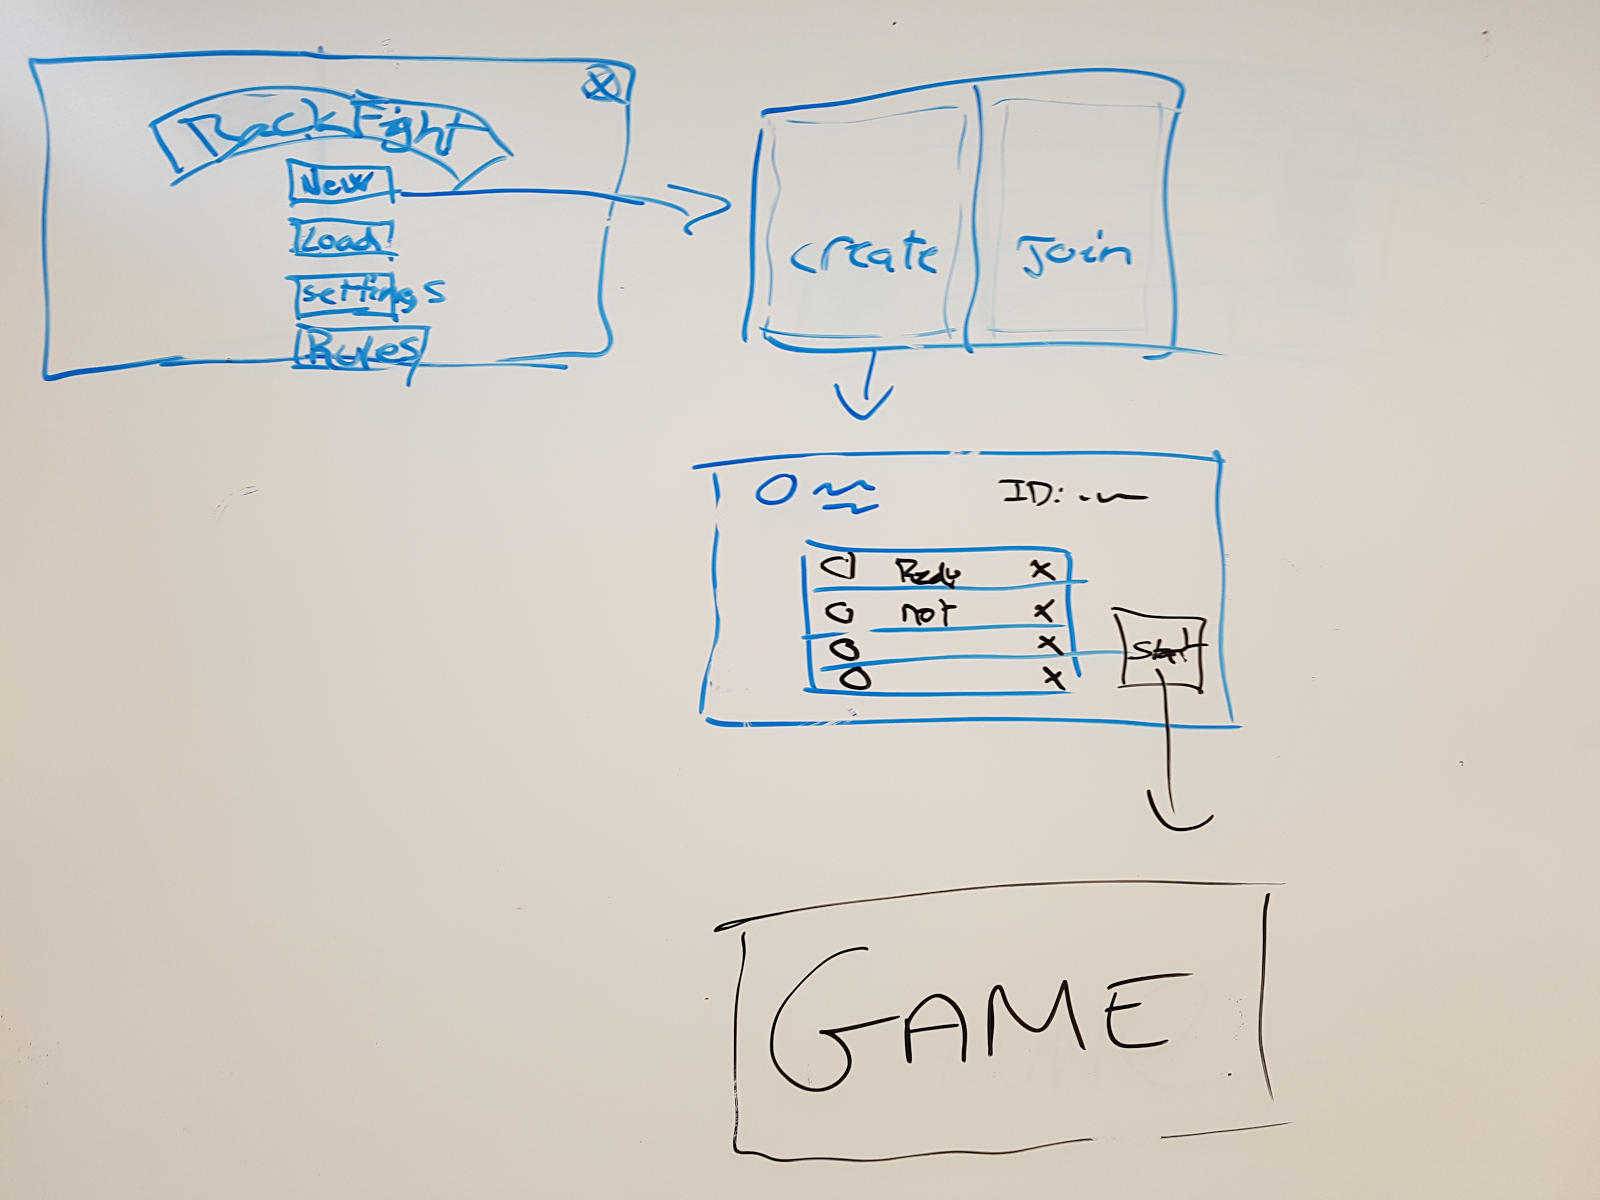
\includegraphics[width=0.8\textwidth]{images/Gui.png}
	\caption{Menu navigation \label{navigation}}
\end{figure}


On \ref{gameLayout} the game view is seen as it was original planed it has been changed a bit under development but the idea of using tiles and players is still the same. There has been added some text to describe rounds and actions left.

\begin{figure}
	\centering
	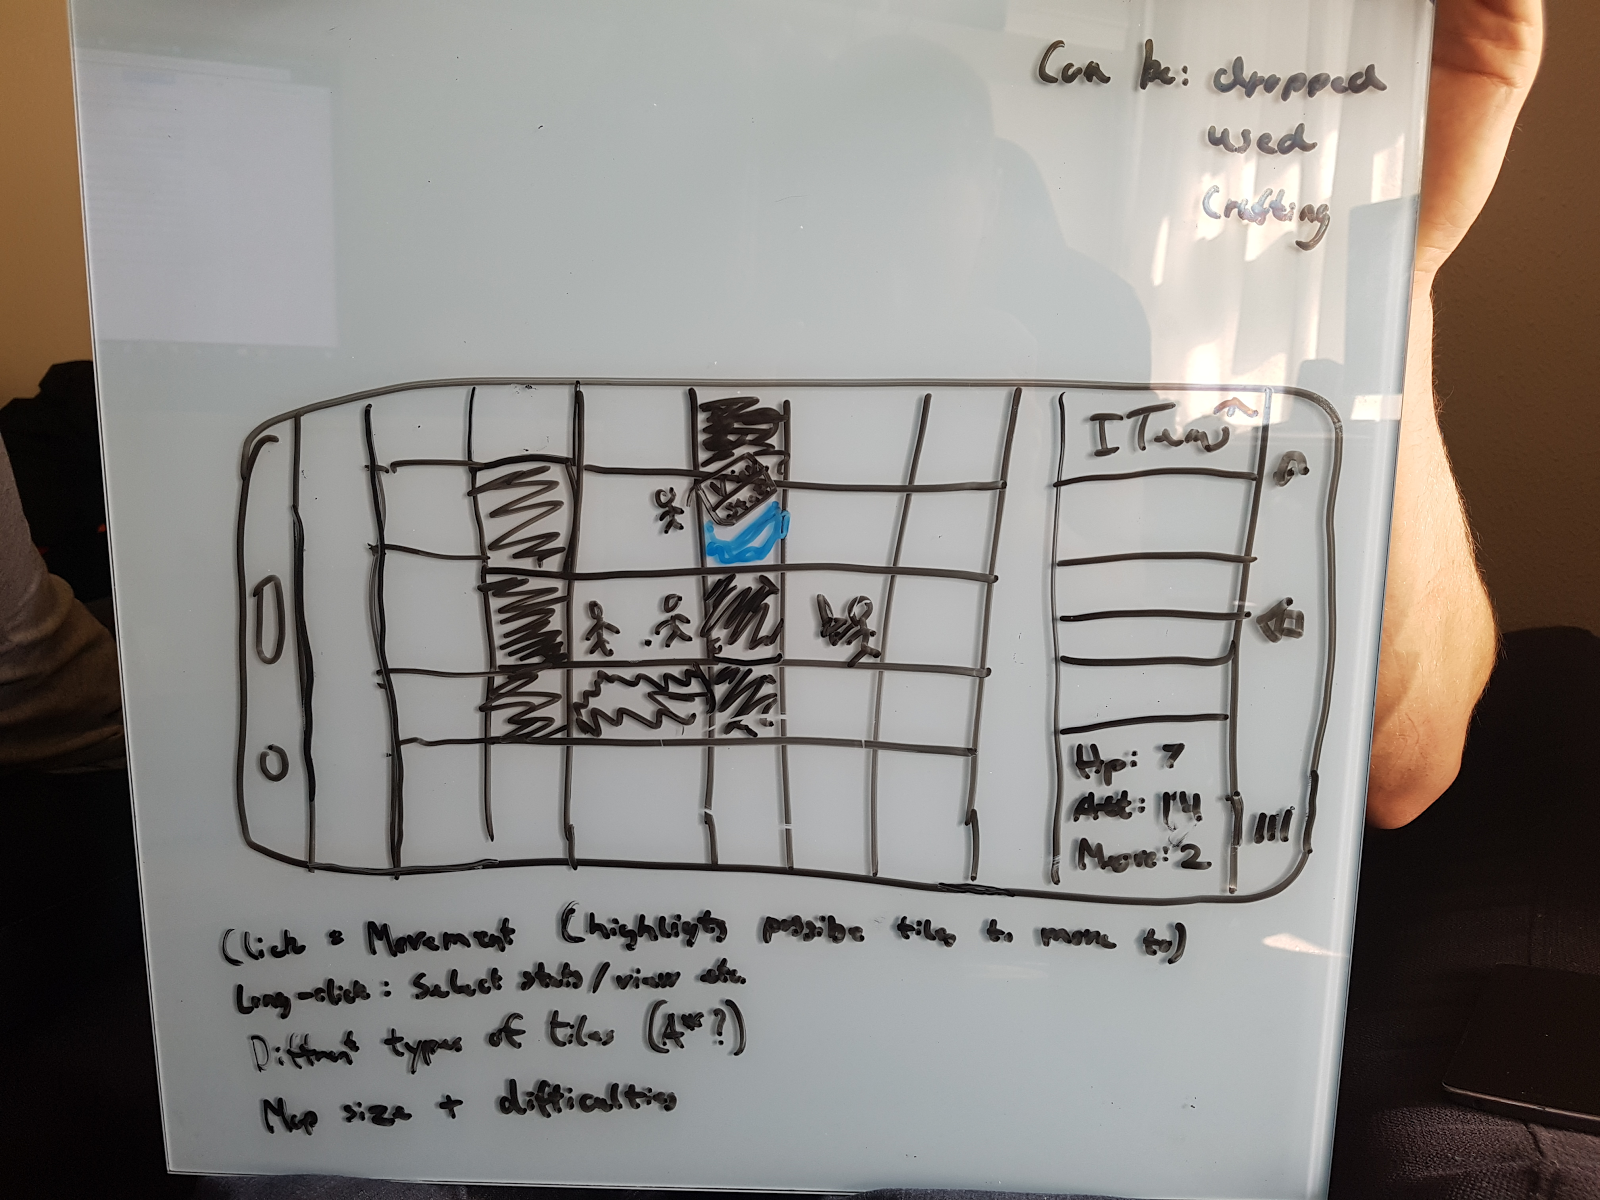
\includegraphics[width=0.8\textwidth]{images/GameView.png}
	\caption{Game layout \label{gameLayout}}
\end{figure}










\pagestyle{Uni}

\chapter{Known Bugs}

\section{Bug List}

\begin{enumerate}
	\item \textbf{Monster spawn:} There is a change that monsters spawn on the same tile as the players when the game starts.
	
	\item \textbf{Kill monster:} When a monster is killed by a player on a tile and another player decides to move to that tile the two players will end up on the same place on that tile. This is because the tile holds 1 player and the tile doesn't know that the player is placed on space 2 and not space 1.
		
	\item \textbf{Spectate:} When spectating a game you have been playing in earlier you will join this game as the player and be able to move yourself. You will also miss some of the normal join features. This should be fixed so the player was informed that they are joining the game as a player.

	\item \textbf{Firebase lag:} When multiple players are making an action at the same time Firebase will reject one of the changes and rollback. This is because the whole list is uploaded instead of just the element in the list that is changed. The game state is split over three lists to minimize the risk of conflicts. This will sometimes create weird scenarios where one of the lists gets updated and the other gets rolled back.
	
	Problem is described here: "If all of the following are true, it's okay to store the array in Firebase\footnote{https://firebase.googleblog.com/2014/04/best-practices-arrays-in-firebase.html}
	
	\begin{itemize}
		\item \textbf{only one client is capable of writing to the data at a time}
		\item to remove keys, we save the entire array instead of using .remove()
		\item we take extra care when referring to anything by array index (a mutable key)"
	\end{itemize}
	In Backfight the game state lists can be changed by multiple users at the same time. To solve this problem either the game could be changed to be round based so each the each user would have a turn. Another solution would be to make some server side logic that would take the changed elements and then handle the synchronization with the database.
	
\end{enumerate}

\pagestyle{Uni}

\chapter{Architecture}

\section{Class Diagram for movement}

On \ref{ClassDiagramMovement} the simplified class diagram is shown it shows how moving a player works. The central part of the diagram is the GameView which is holding the game state lists. These lists control where players, monsters and items are on the map. Each class displayed holds a greater number of functions and attributes but they have been cleared for simplicity, showing only the relevant things for movement and general understanding.


\begin{figure}
	\centering
	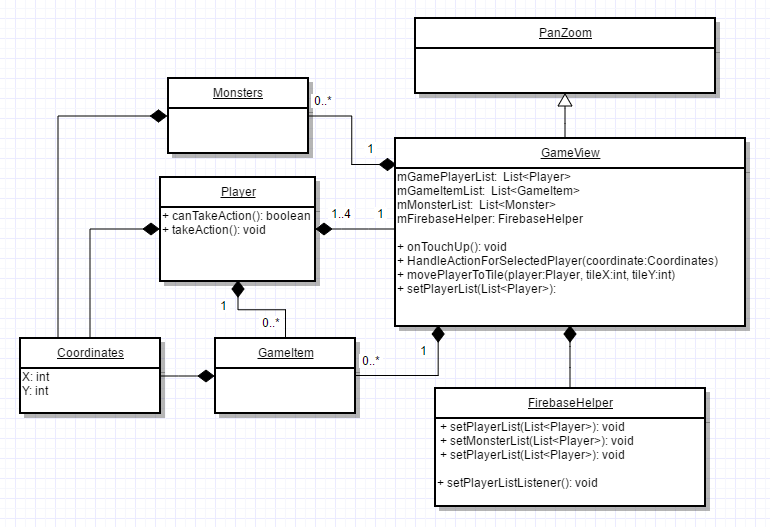
\includegraphics[width=0.8\textwidth]{images/ClassDiagramMovement.PNG}
	\caption{Class Diagram for movement of player \label{ClassDiagramMovement}}
\end{figure}

\section{Sequence Diagram for movement}

On \ref{SquenceDiagramMovement} the sequence of what happens when a person moves the player(avatar) on the screen. Before the player can be moved it is checked if the player got any actions left. The GameView will call the FirebaseHelper where it sets the newly updated PlayerList. This will then get updated asynchronously towards the database. 
Every player have then earlier made an eventListener that listens for changes, so when the database is changed all boards update automatically, by invoking setPlayerList on GameView.

\begin{figure}
	\centering
	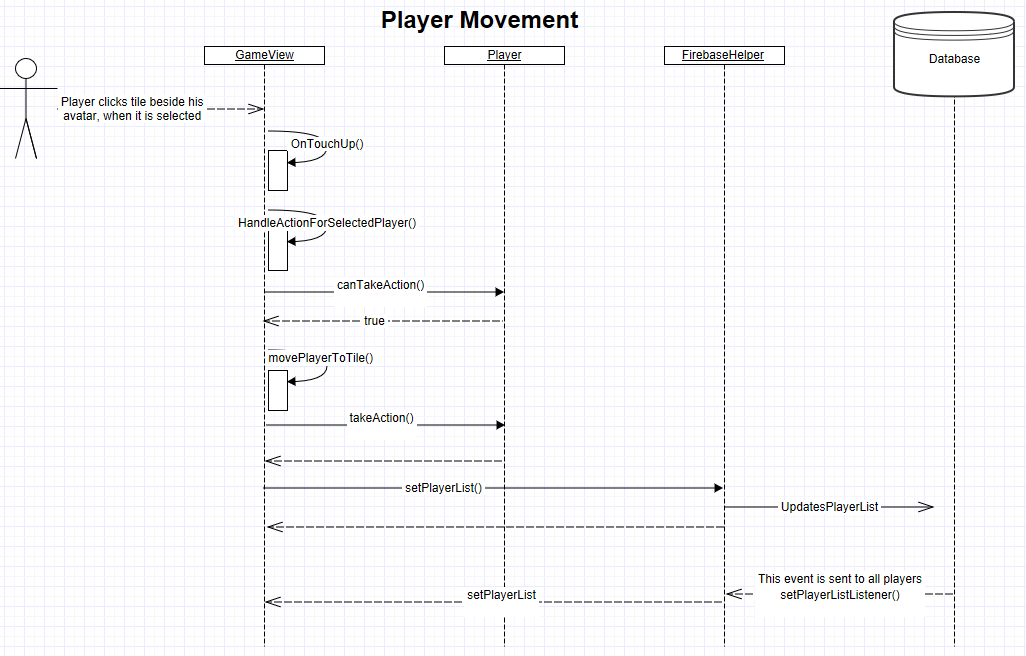
\includegraphics[width=0.8\textwidth]{images/SquenceDiagramMovement.PNG}
	\caption{Sequence Diagram for movement of player \label{SquenceDiagramMovement}}
\end{figure}

\section{Sequence Diagram for start game}

On \ref{SequenceDiagram}the sequence of how to create a new game. The flow shown shows how to create a single player game, but another player can easily join then the host is in the lobby. The flow is simple but need some user input to be completed. The fastest way to create a game and start it takes four user input including opening the app.

\begin{figure}
	\centering
	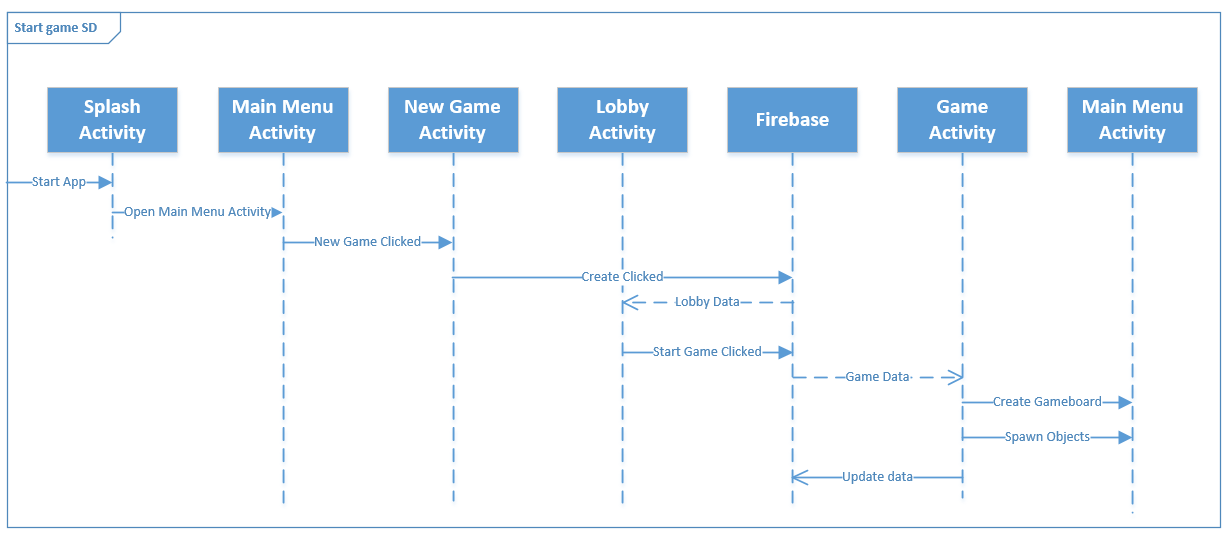
\includegraphics[width=0.8\textwidth]{images/Start_Game_Sequence_Diagram.png}
	\caption{Start Game Sequence Diagram \label{SequenceDiagram}}
\end{figure}

\section{State machine for menu}

On \ref{StateMachine} the state machine shows of how the  menu works, it shows how the flow is and how the user can navigate to the different states. The app starts on a splash screen there is showed for 6 seconds and open the main menu. From the main menu the is a lot of options for the user to do e.g settings and rules. The central part of the diragram is to show how a user can navigate between the different activities and the flow of the app.

\begin{figure}
	\centering
	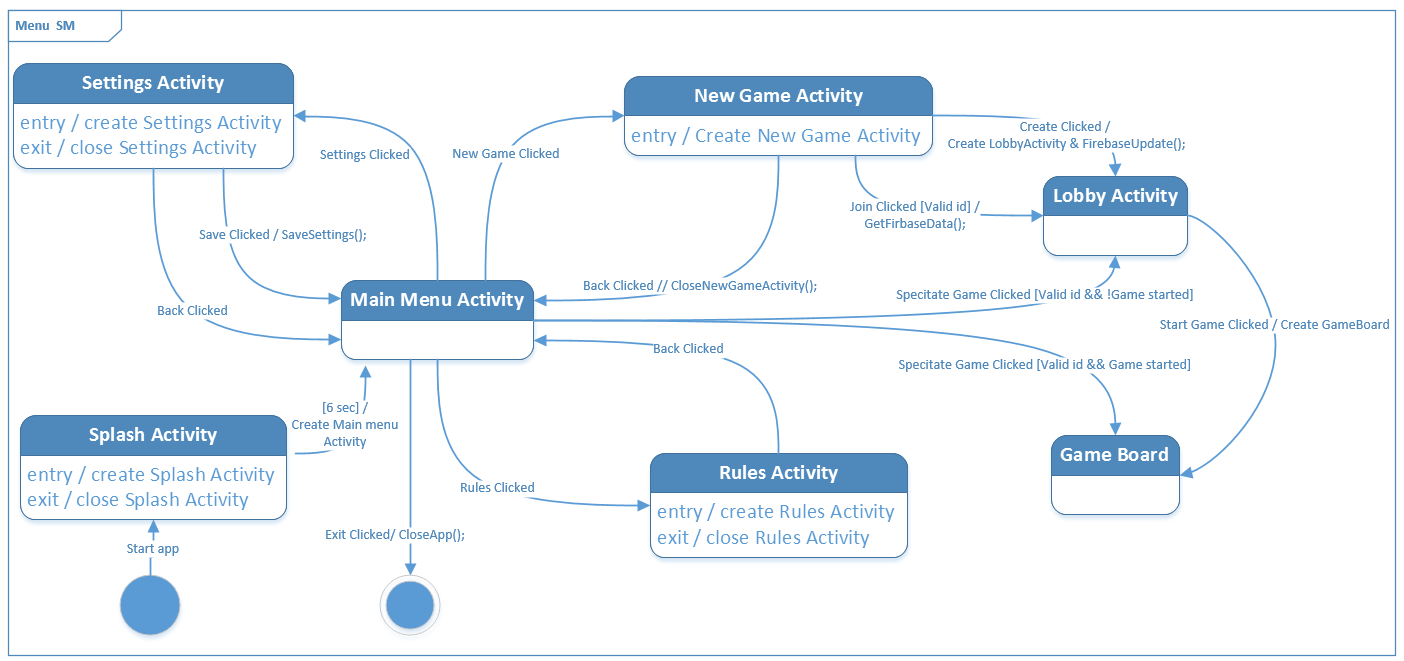
\includegraphics[width=0.8\textwidth]{images/Menu_State_Machine.png}
	\caption{Menu State Machine \label{StateMachine}}
\end{figure}


\chapter{Features}

\section{Firebase}

Firebase is a realtime database, everything is stored as JSON and synchronized in realtime to every connected phone\footnote{https://firebase.google.com/docs/database/}.

The reason for choosing Firebase over any other database was the fast setup, where we in a very short time could setup a database that could fit our needs. The database needed should be able to sync between multiple clients playing a co-op game. It was also handled by the framework and therefore already tested. Firebase is used for everything the requires synchronization between devices and works for controlling the game state.

The use of Firebase in Backfight is described in the following:
Firebase is used for holding game state information to control our game from server side:
The Grid is created when a host presses create it is then distributed to all the users who have joined.
\\
The game state is defined by three different lists and a round count the player list, the monster list and the item list that together defines what state the game is in. These three lists can be changed by all users when they move, attack or pick up items, each of these lists would then change to reflect the action. This allows the other users to see the action on their local device.
\\
The round count is to see what round the game is in this can be used to control difficulty of monsters and events. There is also a shadowed list that holds all the tiles that have been in range of a player that should be shadowed for players unless someone is in range.

There are also lists for the lobby state, since when the host changes settings or start the game these should be reflected on the joined devices.

\section{Items and Monsters}

Items and monsters works in many ways the same even though monsters also share some common traits with the player class.
Both monsters and items has a title/name, description etc.

\begin{figure}[ht!]
	\centering
	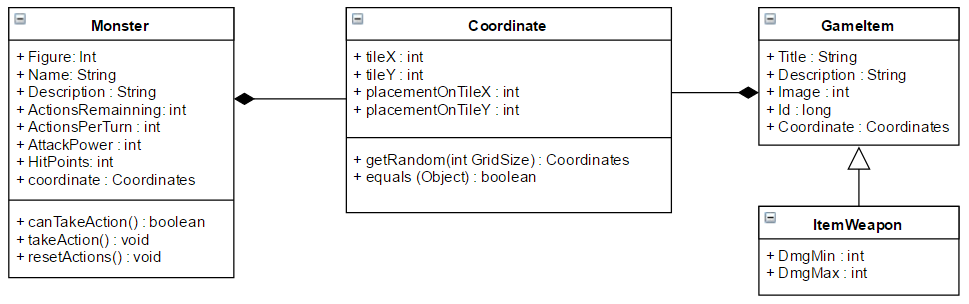
\includegraphics[width=130mm]{images/itemsAndMonstersDiagram.png}
	\caption{Class diagram for monsters and items - Constructors, Getters and Setters has been left out}
	\label{fig:itemsAndMonstersDiagram}
\end{figure}

In the first version of the game neither Monster nor GameItem had Coordinate as a property. Instead it was a list of tuples. The tuples consisted of a monster or game item and a coordinate. It however turned out to be quite difficult to work with, since one had to loop through the list of tuples quite a lot just to get the right monster. It also made it difficult to update the game state, due to these looping and parsing of tuples in methods instead of the monster or game item object. Therefore we changed it to the design shown on figure \ref{fig:itemsAndMonstersDiagram}. When a player picks up an item the coordinate property of that item is then set to null. \\

\subsection{Factories}
Both items and monsters are created via a factory. When creating a monster or item, the gameview request a random item or monster. Currently items are totally randomized and monsters are separated into class'. See "Future Improvements" for more information about future ideas and improvements.


\pagestyle{Uni}

\chapter{Improvements}

Since the application was developed in a very short period of time there are some improvements that could benefit the application. This chapter will list some ideas for these improvements.

\section{Monster drops items}
The team like the idea of items scattered around on the map, but would also like monster to have a chance to drop items when they are killed. Since some items are better than others a looting system in some format would be required.

\section{Monster and item class type}
It is currently possible to spawn three different monster class': 'Common', 'Epic' and 'Boss'. However, the class type is only known at spawn time. As soon as the monster is in the list there is no way to check the class type unless one checks on the name. \\
The same problem is present for items, but here one can't even spawn class type, since it's currently totally random. Therefore it would benefit the gameplay experience to serve the class type info to the player via the fragment (See figure \ref{fig:classTypeCommon} and \ref{fig:classTypeLegendary}). This will also give some better balancing options for the game in case we introduce monster drops etc. so the chance of getting a legendary item is less likely than a simple common sword.

\begin{figure}[ht!]
	\centering
	\begin{minipage}[b]{0.48\textwidth}
		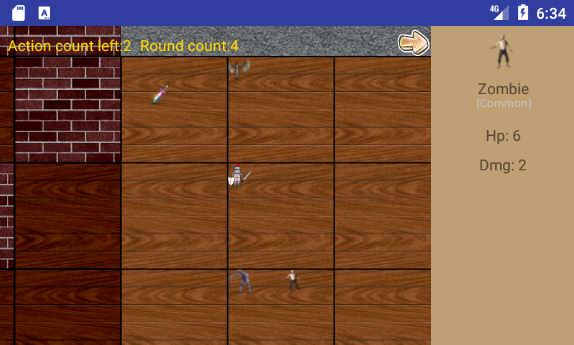
\includegraphics[width=\textwidth]{images/ClassImprovementCommon.png}
		\caption{Common monster}
		\label{fig:classTypeCommon}
	\end{minipage}
	\hfill
	\begin{minipage}[b]{0.48\textwidth}
		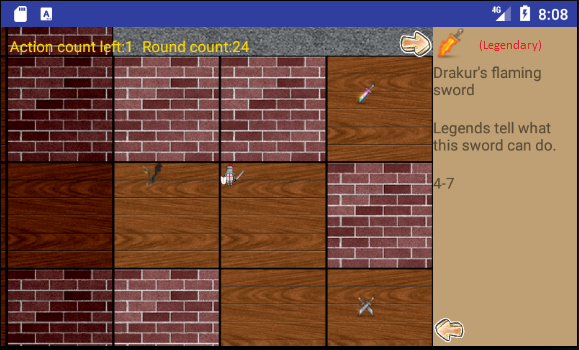
\includegraphics[width=\textwidth]{images/ClassImprovementLegendary.png}
		\caption{Legendary weapons}
		\label{fig:classTypeLegendary}
	\end{minipage}
\end{figure}

\section{Update fragment automatically}
When a player losses health or gain a new item the fragment does not reflect this automatically. Currently, the player has to reopen the fragment in order to get that information. An obvious improvement would therefore to make this happen automatically.\\
This could be done in two ways. Either a similar approach as the item listener, were the activity has the responsibility to update the fragment, or by letting the fragment implement a local broadcast receiver and thereby moving the responsibility into the fragment itself. The last one is the preferred way, since it would make the activity responsible for knowing what to show, but let the fragment be responsible for keeping it up to date.

\section{Different types to items}
The current game only has weapons as items. However, more items will be included in the future. This is also the reason that ItemWeapon class inherit from GameItem class as shown in figure \ref{fig:itemsAndMonstersDiagram}. An example would be armor, that therefore also would inherit from GameItem class.

\section{Firebase synchronisation}
When two or more players take an action at the same time only one would actually take place, the rest would reset their actions. This is both quite annoying for the users but it also introduces some potentially errors since each game state list is maintained asynchronously and separately; One list might get updated correctly, but the others reset. This bug/feature are explained in depth in chapter \ref{ch:knownBugs}. 

%\startcontents[dokumentation]
%\renewcommand{\baselinestretch}{0.75}\normalsize
%\printcontents[dokumentation]{ }{0}{\chapter*{Indholdsfortegnelse}}
%\renewcommand{\baselinestretch}{1.1}\normalsize


%Bibliography
%\bibliography{Dokumentation/bibtex/litteratur}


%\stopcontents[dokumentation]

\end{document}
